% !TeX spellcheck = en_US
%\documentclass[11pt,a4paper]{article}
\documentclass[11pt
  , a4paper
  , article
  , oneside
%  , twoside
%  , draft
]{memoir}

\usepackage{control}
\usepackage[numbers]{natbib}

\newcommand{\newappendix}{%
  \refstepcounter{chapter}\chapter*{Appendix \thechapter}%
  \addcontentsline{toc}{chapter}{Appendix \thechapter}%
}

\begin{document}
	
\newcommand{\technumber}{
  RAON Control-Document Series\\
  Revision : v1.0,   Release : January 21, 2016}
\title{\textbf{Configuration of the Demo Vacuum system using AB PLC on the EPICS}}

\author{Hyungjoo Son \\

  Rare Isotope Science Project\\
  Institute for Basic Science, Daejeon, South Korea
}
\date{\today}

\renewcommand{\maketitlehooka}{\begin{flushright}\textsf{\technumber}\end{flushright}}
%\renewcommand{\maketitlehookb}{\centering\textsf{\subtitle}}
%\renewcommand{\maketitlehookc}{C}
%\renewcommand{\maketitlehookd}{D}

\maketitle

\begin{abstract}\
  중이온 가속기에서 모든 제어환경은 EPICS에 통합될 예정이다. EPICS 환경에 로컬 제어시스템을 통합시키기 위해서는 로컬 제어시스템에서 각 디바이스들의 제어에 사용되는 PLC(Programmable Logic Controller)의 데이터들을 EPICS 환경으로 불러오는 과정이 필요하며, 이를 위해 EPICS IOC(Input Output Controller)를 구성하여 PV(Process Value)로 PLC의 데이터 값들을 관리하는 시스템을 구현해야 한다. 
  본 문서에서는 현재 제어실에 구성한 Demo Vacuum System의 제어용 PLC인 AB PLC의 설정 방법 및 PLC 기본 프로그래밍 방법에 대한 소개, 그리고 EPICS 환경에 AB PLC를 통합시키는 방법과 제어환경 모니터링을 위한 UI(User Interface) 시스템을 구성하는 방법에 대해 기술할 것이다.
\end{abstract}

\chapter{Demo Vacuum System의 구성}\
Demo Vacuum System(DVS)는 크게 장치부와 제어부로 나눌 수 있다. 장치부는 챔버를 진공환경으로 만들기 위해 장착되는 TMP(Turbo Molecular Pump)와 각종 디바이스를 말한다. 제어부는 TMP controller 및 Gauge controller와 데이터 교환을 통해서 DVS의 디바이스들을 제어하는 동시에 모니터링하는 시스템을 말한다.

\section{장치부 구성}\
다음은 DVS에 설치되어 있는 디바이스들이다. TMP는 현재 ECR Ion Source 모듈에 설치된 OSAKA TMP이며, 게이지 컨트롤러 또한 같은 환경에서 사용하는 제품이다.

\begin{itemize}
\item Turbo Molecular pump 	: OSAKA TG450FCAB
\item TMP Controller	    : TC-353
\item Convection Gauge(CG)  : Convec Torr P-type
\item Pull range Gauge      : FKG-730
\item Gauge Controller      : XGS-600
\item Gate Valve            : SSE51200
\item Angle Valve           : SSEPBK025A
\item Dry pump				:IDP-15
\end{itemize}


\section{제어부 PLC 구성}\
다음은 위에서 구성한 디바이스들과 와이어링을 통해 디바이스들을 제어하고 데이터들을 교환하기 위한 AB(Allen Bradly) PLC의 구성이다. 실제 로컬사이트에서 제어해야 할 장비들과 거리 및 제어환경을 고려해서 Remote 환경으로 구성하였으며, 대부분의 로컬 시스템의 기본구성인 디지털 모듈, 아날로그 모듈, 시리얼 통신 모듈을 장착하였다.

\begin{itemize}
\item PLC CPU	 			: L30ER
\item Digital Input card	: 1769-IQ16 (Sink/Source) 
\item Digital Output card	: 1769-OB16 
\item Analog Input card		: 1769-OF2 
\item Analog Output card	: 1769-IF4 
\item Serial communication card	: 1734-232ASC 
\item Remote IO module			: 1734-AENT Point IO 
\end{itemize}

PLC CPU는 Compact type인 CompactLogix 모델로 구성하였으며, 로컬 사이트에서 주로 사용되는 Control Logix 보다는 확장성이 좋지는 않지만, 기능상으로는 거의 동일하게 시스템을 구성할 수 있고 가격적인 장점이 있어서 Test PLC로 적용하였다.\\
디지털 입력카드의 경우는 거의 대부분이 센서와 연결이 되는 경우가 많으므로 디지털 입력카드에 따라 센서의 종류를 NPN형 및 PNP형으로 선택하는 것이 추후 전장 패널구성 시 용이할 것이다.\\
Remote 모듈의 경우는 LAN으로 연결만 되면 IP address를 부여하여 추가로 카드를 설치할 수 있어서 전장 패널을 구성함에 있어서 제약이 없다는 장점이 있다.\\
Serial communication 카드는 Remote 모듈에 장착하여 사용할 수 있으며, Serial 통신의 거리 의존성으로 인해 가능하면 통신할 controller와 가까이에 설치하여 사용하는 것을 권장한다.
\\
\newline
Figure 1은 현재 구성된 Vacuum testbed의 개념도이며, Figure 2와 3은 실제 설치된 PLC와 DVS이다.\\

\begin{figure}[!htb]
  \centering
  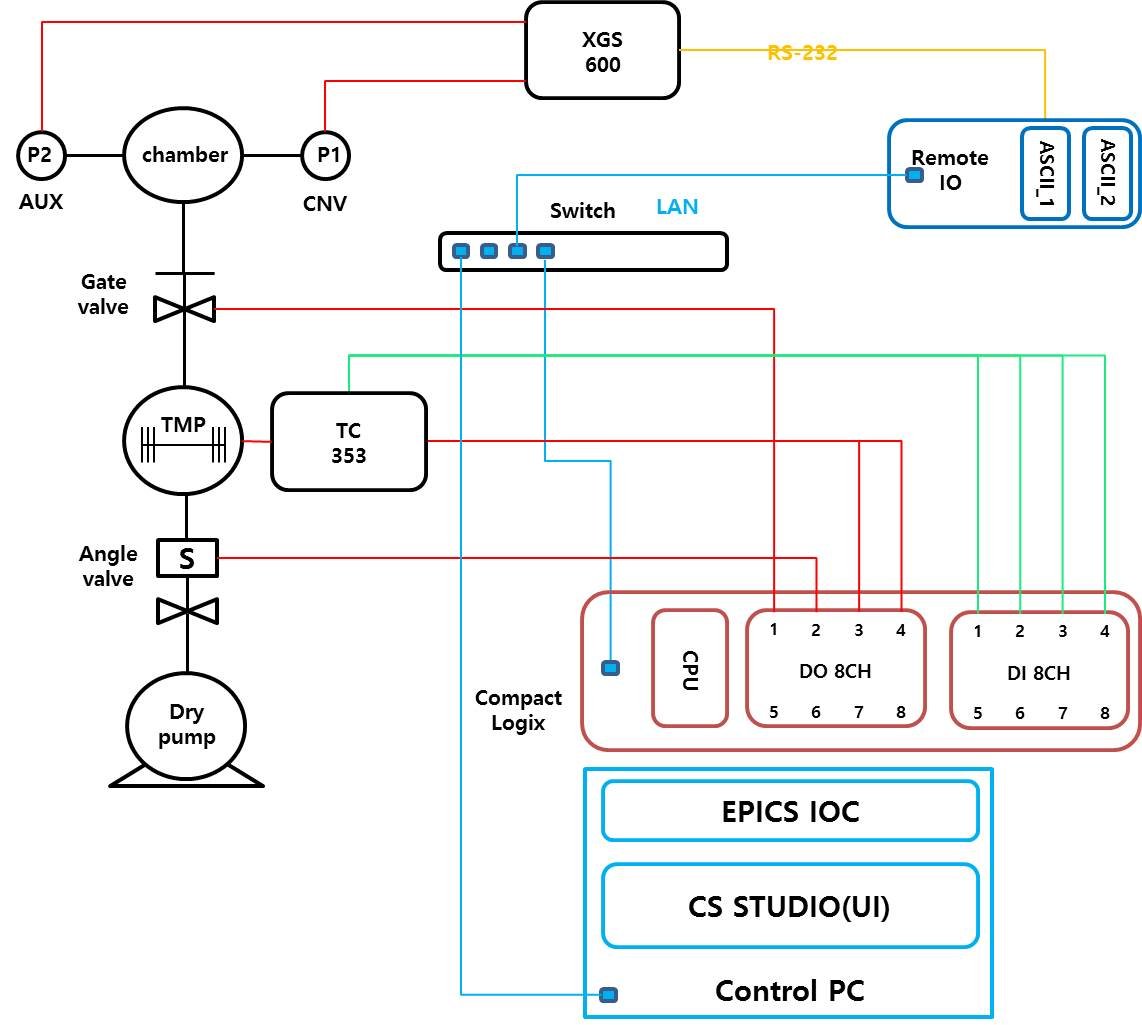
\includegraphics[width=1 \textwidth]{./picture/configuration_diagram.jpg}
  \caption{
             Diagram of the DVS
          }
  \label{fig:}
\end{figure}

\newpage

\begin{figure}[!htb]
	\centering
	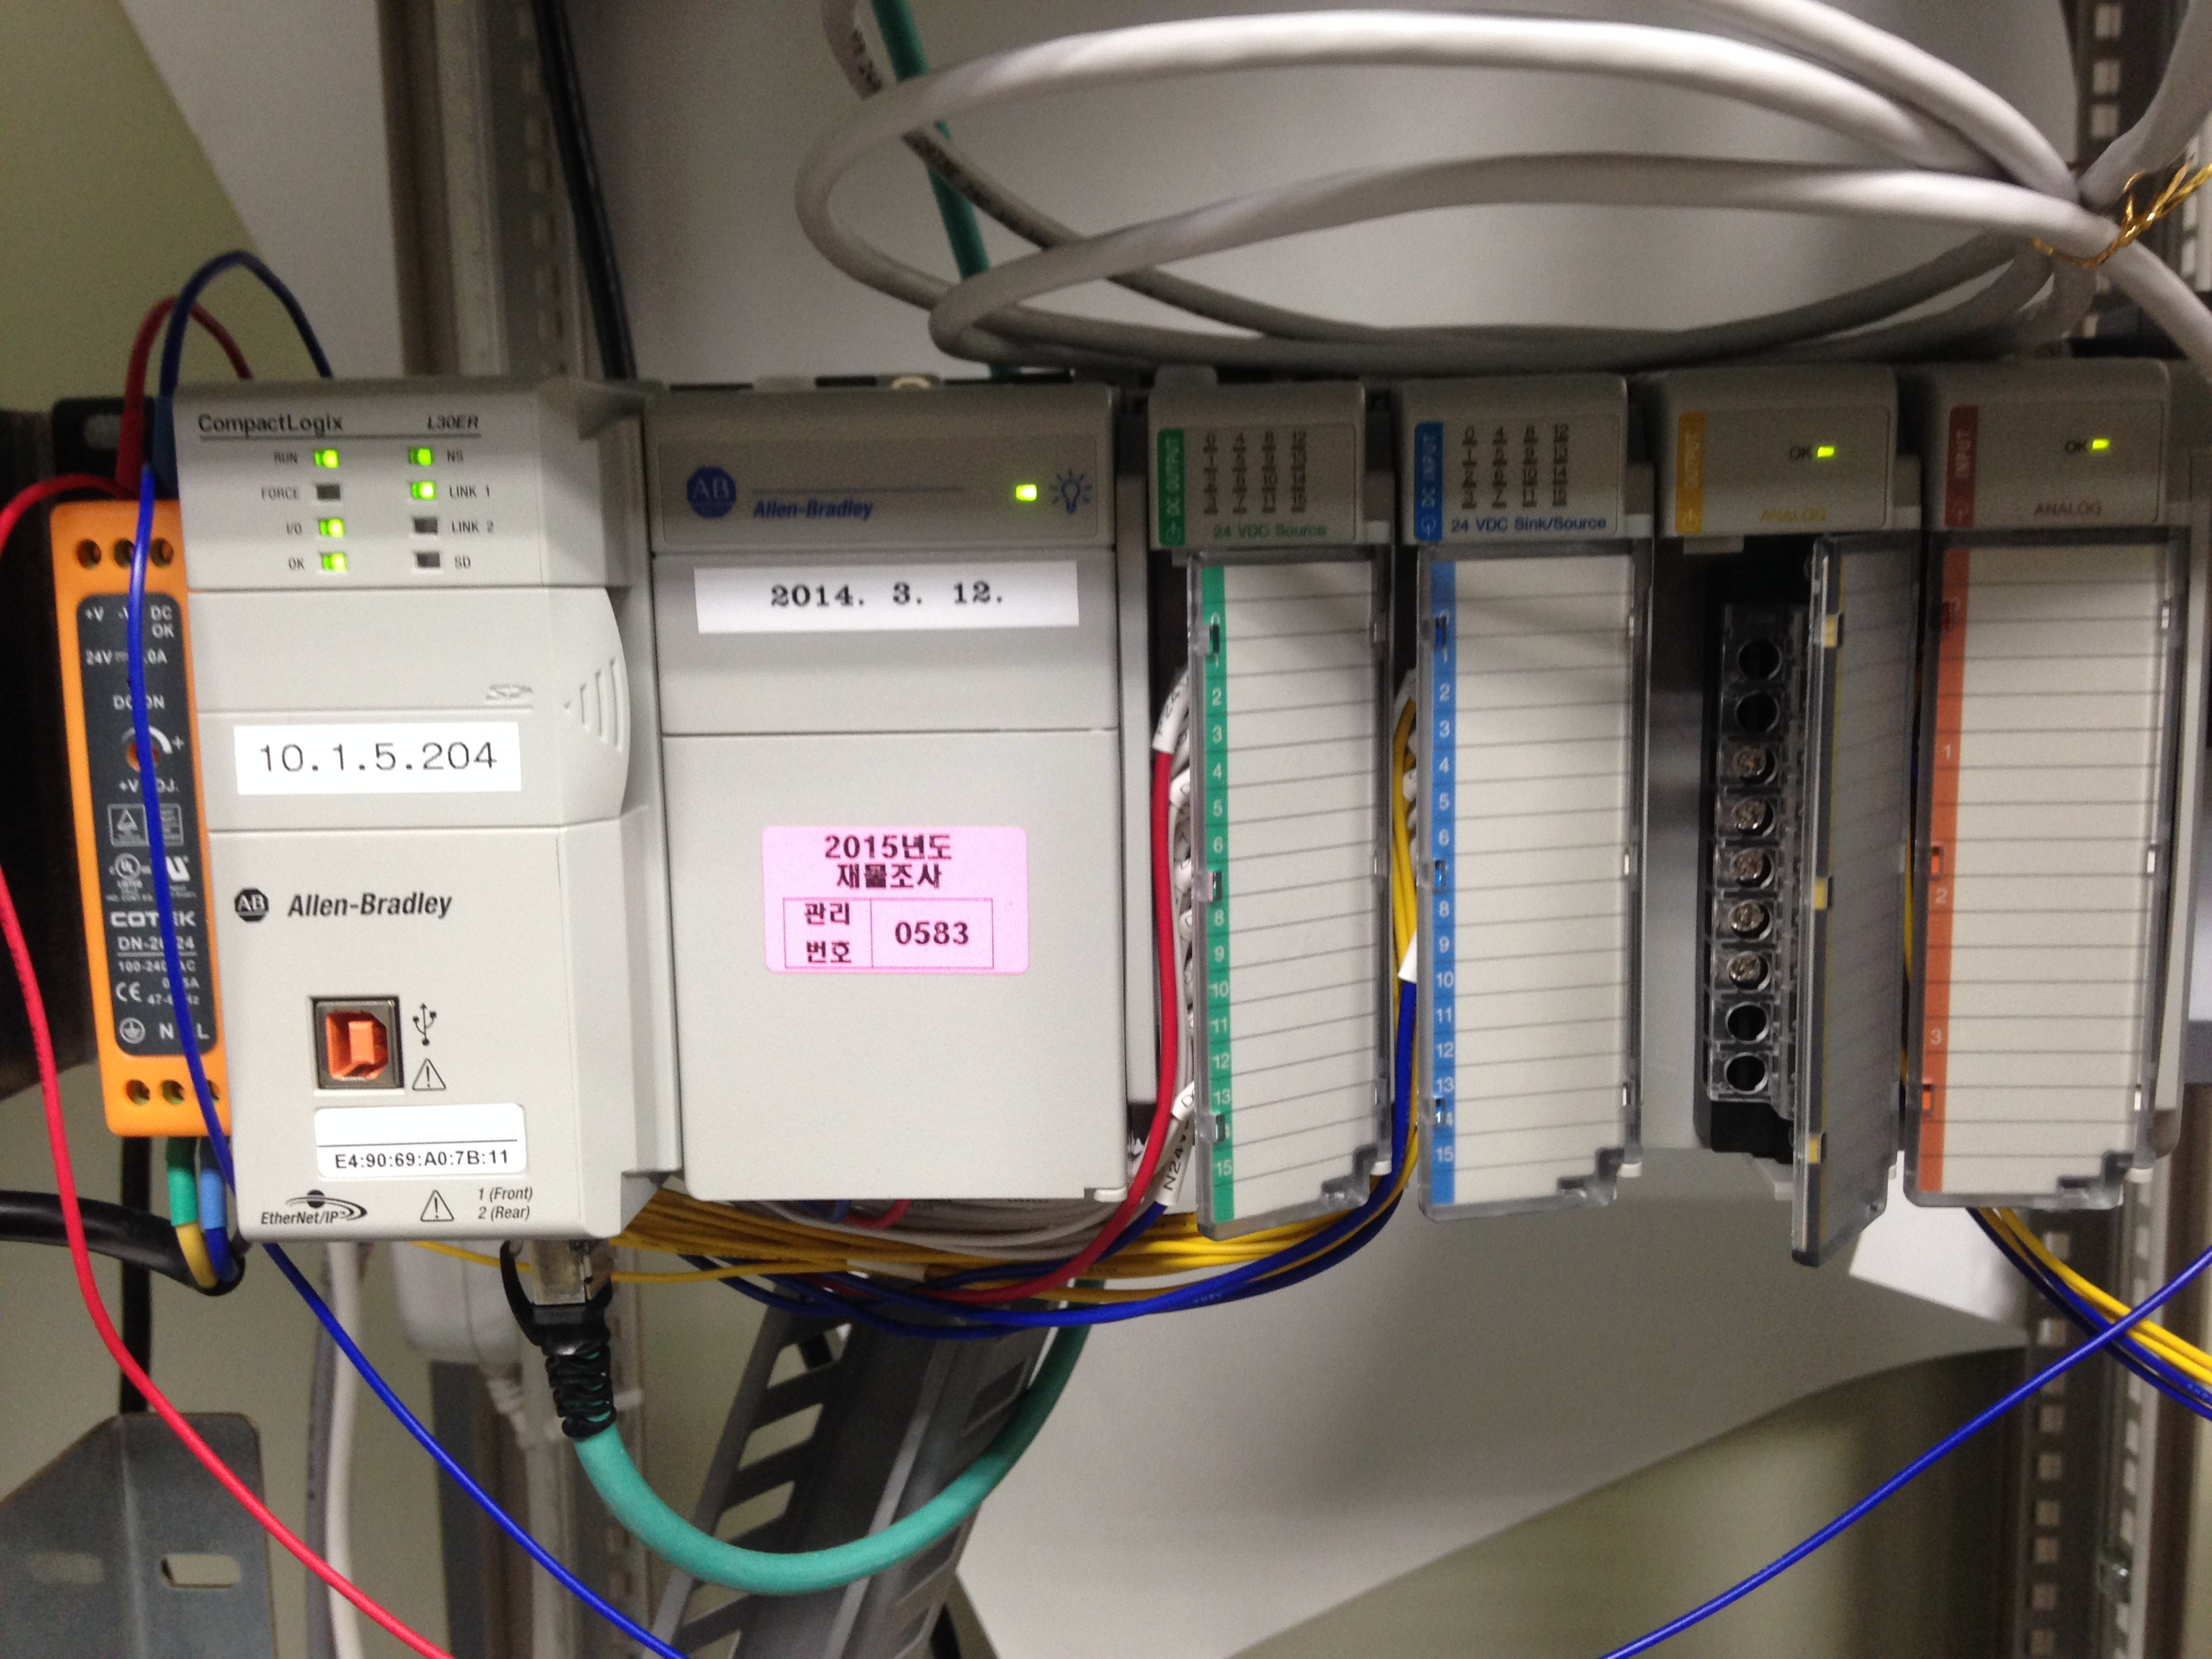
\includegraphics[width=0.8\textwidth]{./picture/compact.JPG}
	\caption{
		CompactLogix PLC 
	}
	\label{fig:}
\end{figure}\

Figure 2에 나타나 있듯이 AB PLC는 라벨의 색깔에 따라서 그 모듈의 특성을 알 수 있다. 예를 들어 1슬롯에 꽂혀 있는 녹색 라벨 모듈의 경우는 Digital Output을 말하며, 2슬롯에 꽂혀있는 파란색 라벨 모듈은 그 모듈이 Digital Input임을 나타낸다. 현재 PLC 구성은 Figure 2의 왼쪽부터 CPU, Power, Digital Output, Digital Input, Analog Output, Analog Input 순서로 설치되어 있다.

\begin{figure}[!htb]
	\centering
	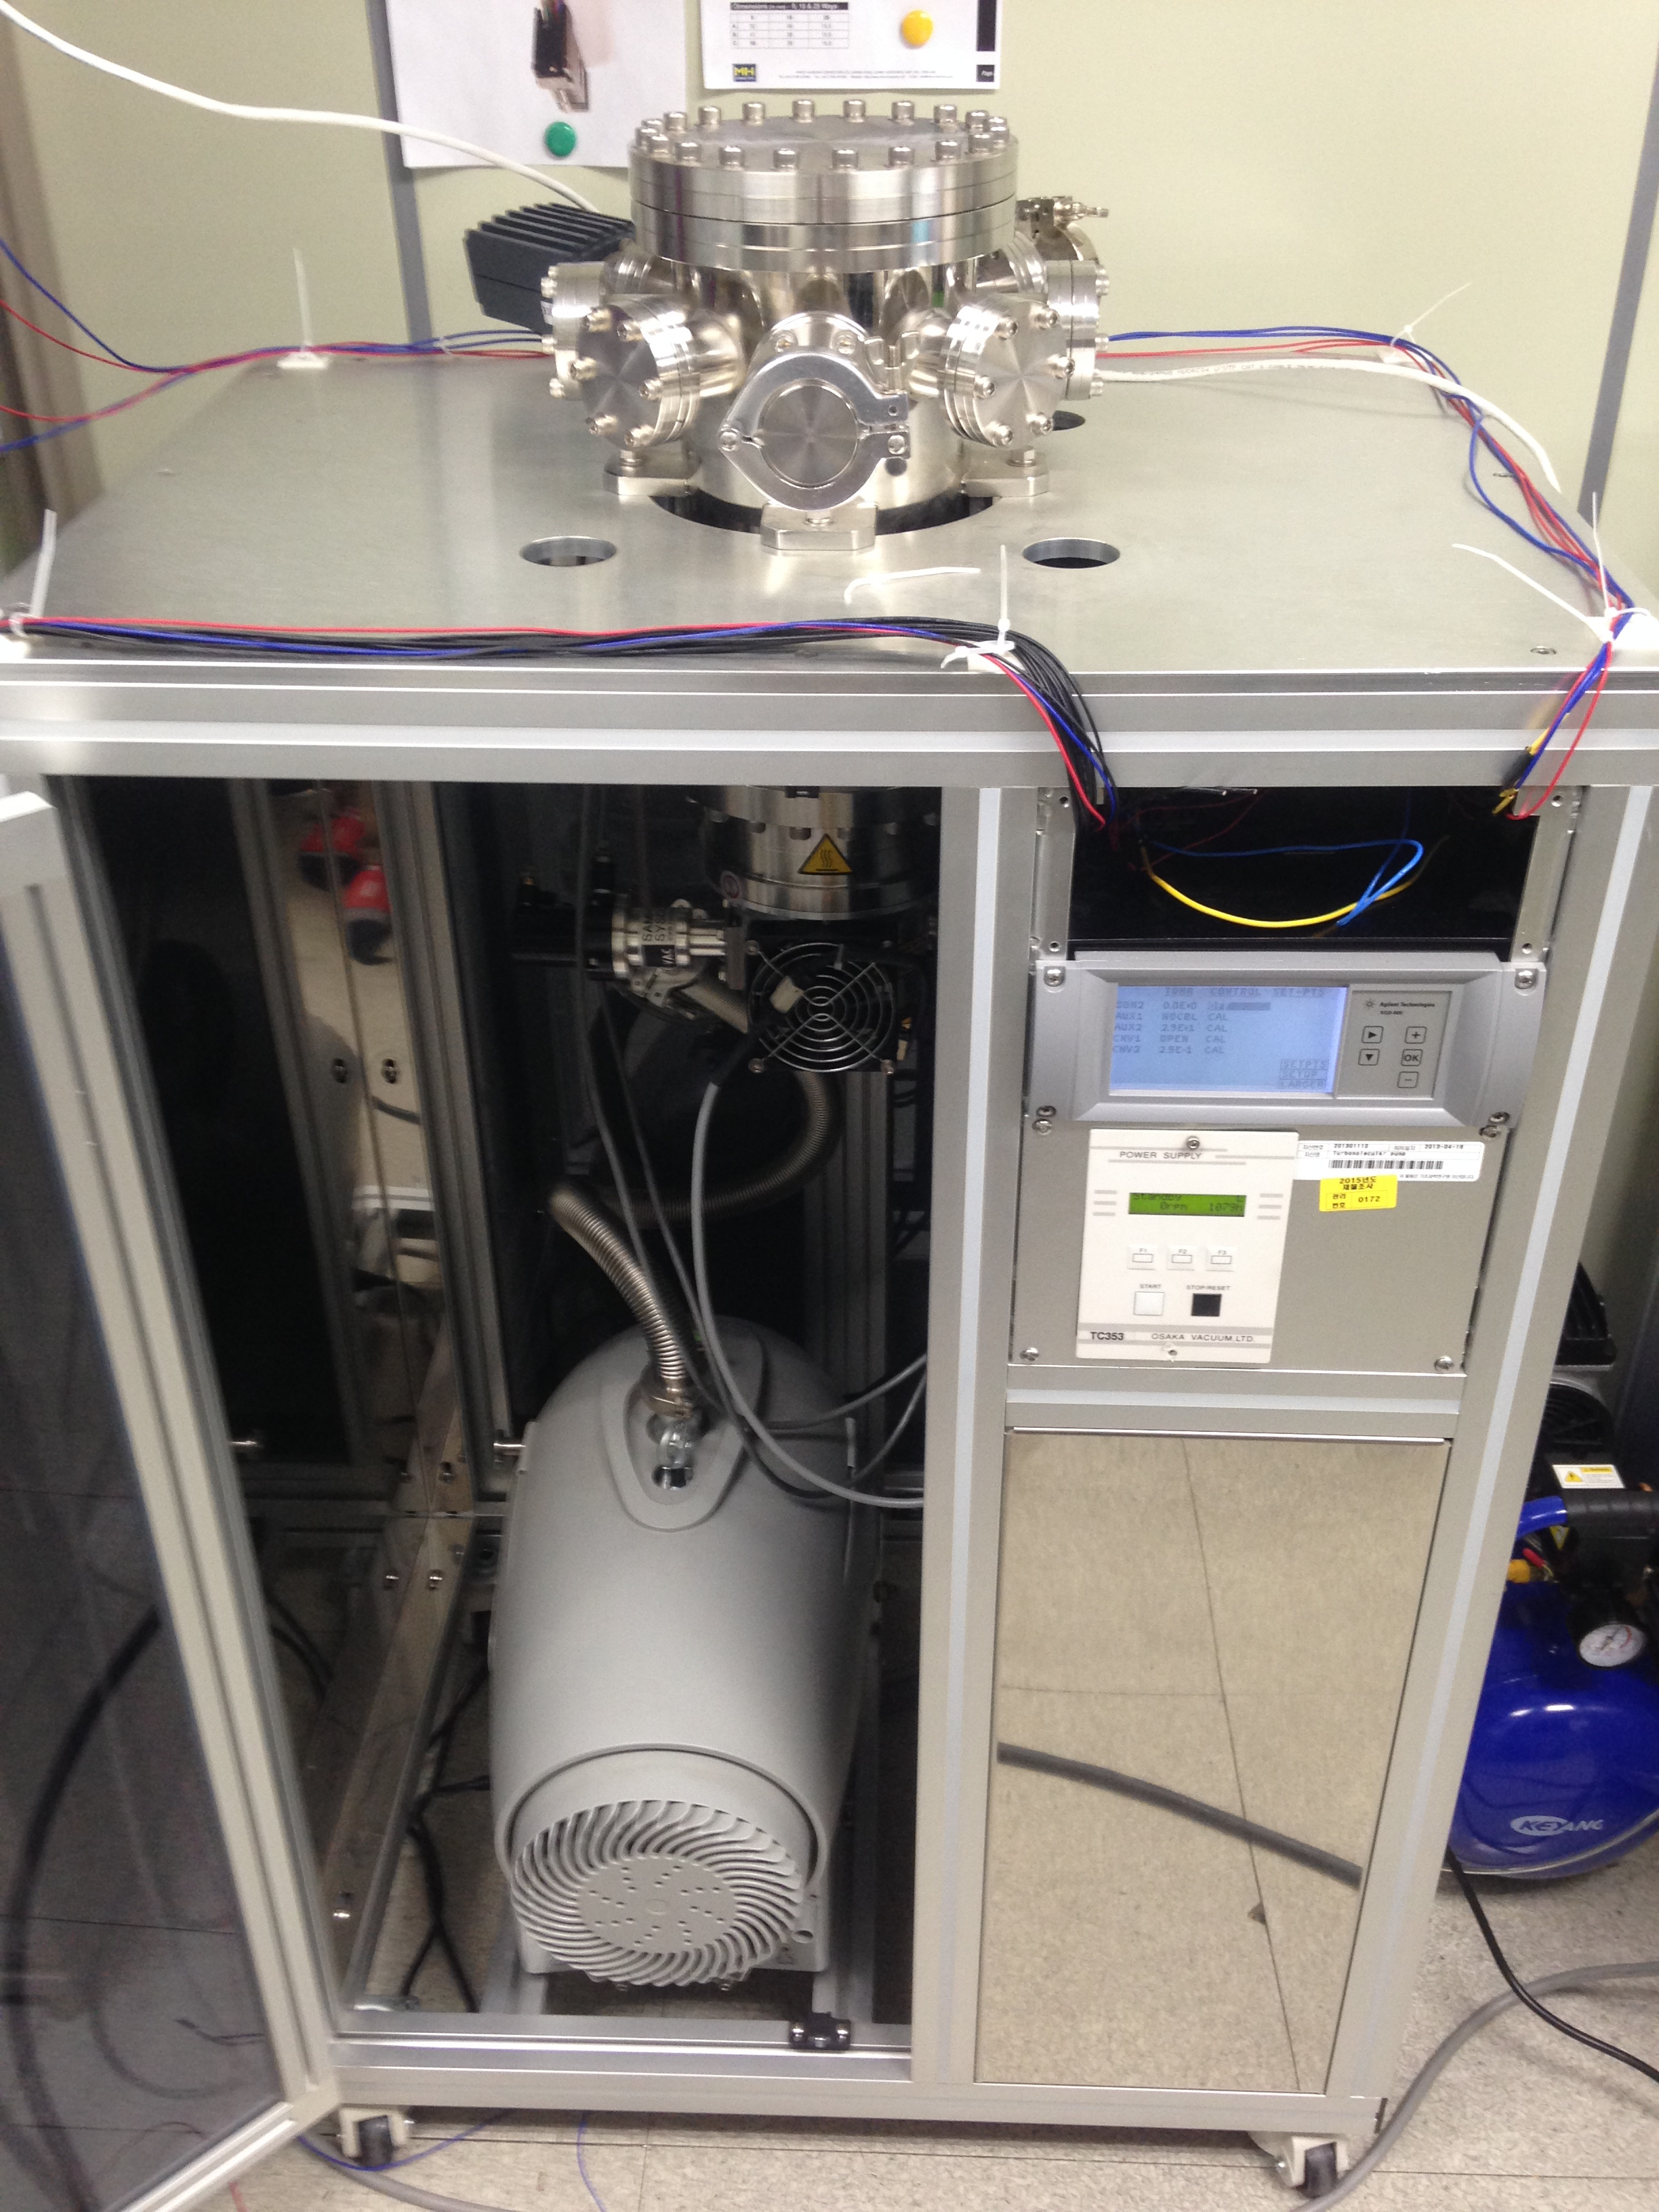
\includegraphics[width=0.6\textwidth]{./picture/vacuumsystem.JPG}
	\caption{
		Vacuum testbed
	}
	\label{fig:}
\end{figure}

\newpage

\chapter{AB PLC Progarmming}\
 여타 PLC와 마찮가지로 AB PLC는 스크립트 형태로 프로그래밍 하는 ST(Statement), 입출력 및 명령어를 순차적으로 입력하는 LD(Ladder), PLC 자체에서 명령어에 따라 제공되는 FB(Function Block) 형태의 세 종류의 언어를 사용할 수 있다. 일반적으로 PLC 프로그래밍은 순차 제어를 위해서는 Ladder 방식으로 구성하는 것이 수월하며, PID 제어와 같이 여러 파라미터들을 동시에 확인할 필요가 있는 것들은 FB의 형태로 프로로그램을 많이 작성한다. ST 방식은 이기종 PLC 간의 명령어가 다른 특성에 크게 구애 받지 않는 장점이 있다. 

\section{PLC 입출력 메모리 구성}\
 AB PLC는 메모리 주소를 Tag로 구성한다. Tag의 장점은 해당 메모리 주소값 대신에 Tag name을 부여한 후 데이터 타입만 설정해 주면 되므로 별도의 메모리 주소값에 대한 설명을 써 주지 않아도 되며, 메모리 형태에 따른 메모리 지정 주소에 대한 관리도 필요없다는 것이다. 
 또한 Tag는 Controller Tag와 Program Tag로 구성되는데 이는 일반적인 프로그래밍 개념에서 전역변수와 지역변수로 생각하면 된다. Controller Tag로 설정된 Tag는 전체 PLC 프로그래밍에서 사용할 수 있으나 Program Tag로 설정된 Tag는 해당 Routine 프로그래밍에서만 유효한 값이 된다. EPICS IOC의 PV(Process value)와 연동되기 위해서는 PV에 해당되는 Tag는 Controller Tag로 설정해야 한다. 프로그래밍에 관련된 사항은 뒤에 자세히 설명한다.\
 
 기본적으로 AB PLC 시스템을 구성했을 시 설치된 모듈의 종류에 따라 PLC 자체에서 부여되는 Tag가 Figure 4와 같이 구성이 된다. 아래는 Figure 4에서 보여주는 Tag에 대한 설명이다.  
  
\begin{figure}[!htb]
	\centering
	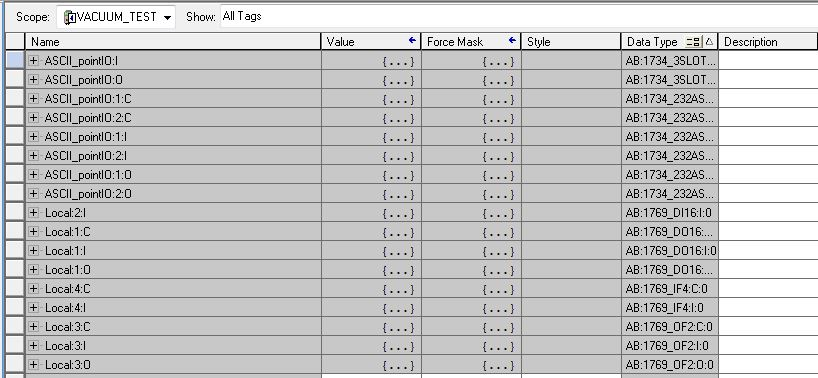
\includegraphics[width=0.96\textwidth]{./picture/tag_local.JPG}
	\caption{
		Tag configuration of AB PLC
	}
	\label{fig:}
\end{figure}  
  
\begin{itemize}
\item Assigned Digital Output memory\\
Digital Output모듈이 슬롯 1에 설치된 경우 Output tag는 Local:1:O 영역에 할당된다. Local은 CPU가 설치된 샤시를 가리키며, 1은 슬롯 번호, O는 Output을 의미한다. Local:1:O의 영역은 Local:1:O.0부터 Local:1:O.15까지 16bit의 bit 정보를 가지고 있다. 
\end{itemize}

\begin{itemize}
\item Assigned Digital Input memory\\
Digital Input모듈의 메모리는 Local:2:I 영역에 할당된다. I는 Input을 의미하며, Local:2:I영역은 출력과 마찮가지로 Local:2:I.0부터 Local:2:I.15까지 16bit의 bit 정보를 가지고 있다. 
\end{itemize}

\begin{itemize}
	\item Assigned Analog Output memory\\
	Analog Output모듈의 메모리는 Local:3:O 영역에 할당된다. Analog 타입의 메모리는 기본적으로 DINT(Double Integer) 타입으로 할당된다. 
\end{itemize}


\begin{itemize}
	\item Assigned Analog Input memory\\
	Analog Input모듈의 메모리는 Local:4:I 영역에 할당된다.
\end{itemize}

AB PLC 의 내부 Tag의 형태는 크게 Timer, SINT, DINT, STRING, BOOL(bit), FLOAT, Double FLOAT 형의 Tag로 나눌 수 있다. 이것은 다른 PLC와 같은 개념이므로 본 문서에서는 직접 프로그래밍에 직접 사용되는 경우를 제외하고는 언급을 하지 않는다.\

\newpage

 \section{PLC Programming software}\
AB PLC를 제어하기 위해서는 기본적으로 두 가지 소프트웨어 툴을 써야한다. 소프트웨어는 네트워크 환경을 구성하기 위한 툴과 실제적인 제어 프로그래밍을 구성하는 툴로 나눌 수 있다. 모든 제어프로그램은 유료이며, 구매한 라이센스를 활성화하는 방식으로 관리되고 있다.(국산인 LSIS는 모든 소프트웨어가 무료임)

RS-Linx는 AB PLC의 IP주소를 설정하여, PLC CPU에 연결되어 있는 모듈들의 정보들과 네트워크에 연결된 모든 디바이스들을 표시해 준다. 초기 IP 설정 방법은 Rockwell 사의 홈페이지(ab.rockwellautomation.com)에서 다운로드 받을 수 있다. 

Logic5000은 설치된 모듈들의 등록 및 모듈 특성 설정,순차 제어 로직을 구성하는 프로그램으로서 입출력 및 다른 디바이스들과의 통신 로직을 구성할 수 있다. Logic5000 역시 매뉴얼을 홈페이지에서 제공하나, 그 양이 방대하고 제어의 목적에 따라 사용하는 명령어가 다르므로 본 문서에서는 기본적인 입출력 구성과 Vacuum Testbed를 제어하기 위해 수행했던 통신설정 등을 위주로 Logic5000의 기능을 설명한다. 기본 모듈 구성은 제조사에서 제공하는 매뉴얼을 참조하기 바란다. 
  
  \section{Network setting and Module configuration}
 PLC 제어환경을 구성하기 위해서는 먼저 RS-Linx 프로그램을 실행하여 PLC CPU의 IP address를 설정한다. Figure 5의 상부 메뉴의 Communication 메뉴를 선택한 후 Who를 선택하면 현재 AB PLC CPU와 같은 네트워크에 연결된 모든 장비를 볼 수 있다. 현재의 상태는 이미 PLC 모듈의 등록과 네트워크 구성이 끝난 상태이다.\\ 
 
 Figure 5의 왼쪽부분에서 제어용PC, PLC CPU, Remote IO의 IP address를 확인할 수 있으며, 그 하위 정보를 통해서 어떠한 모듈들이 구성되어 있는지에 대한 정보를 얻을 수 있다.
 
 
 \begin{figure}[!htb]
 	\centering
 	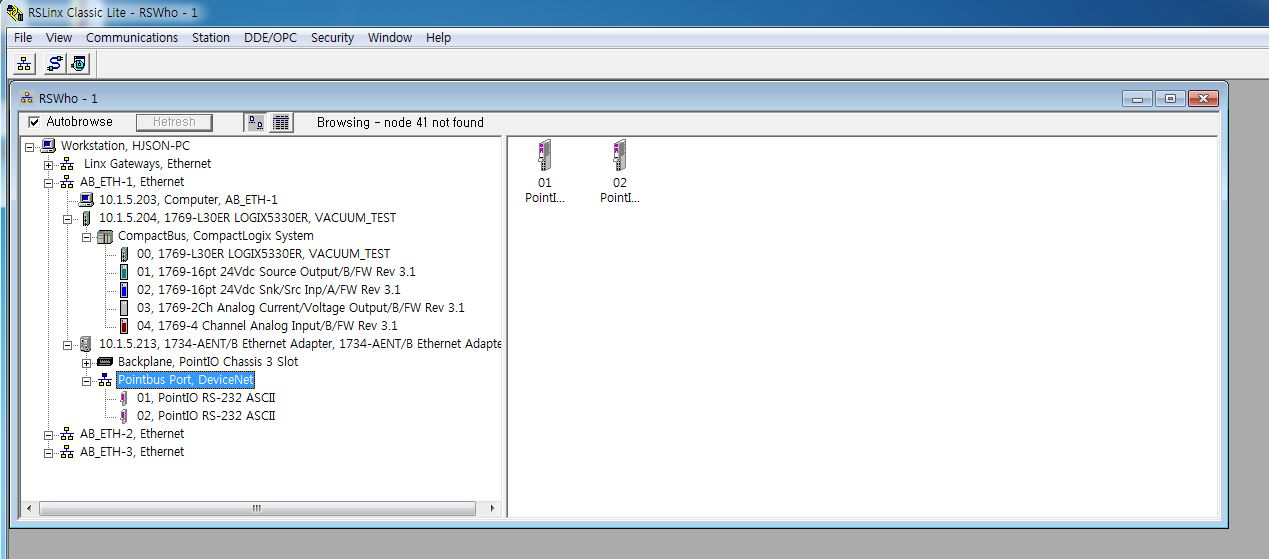
\includegraphics[width=0.96\textwidth]{./picture/rslrinx.JPG}
 	\caption{
 		AB PLC Networking setting
 	}
 	\label{fig:}
 \end{figure}  
 
 \newpage 
 
 Figure 5와 같이 PLC CPU의 IP address 설정이 끝나면 RS-linx 프로그램은 네트워크 상태를 확인하는 용도로만 쓰인다. PLC module의 등록과 래더 로직 프로그래밍은 RSLlogix5000 프로그램을 이용하여 구성한다. 모듈의 등록 및 래더 로직구성법은 아래의 절차를 따른다.\\
 
 1) RSLogix5000을 실행시키면 초기화면의 왼쪽 영역 하단부에 Figure 6과 같은 모듈 등록창이 생성된다.\\
 
  \begin{figure}[!htb]
  	\centering
  	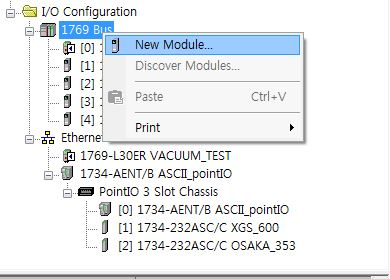
\includegraphics[width=0.7\textwidth]{./picture/module_regi.JPG}
  	\caption{
  		I/O configuration
  	}
  	\label{fig:}
  \end{figure} 
2) CPU 모듈을 우클릭 하면 New Module 메뉴를 선택한다. Figure 7과 같이 모듈 등록창이 팝업된다.\\
 
 \begin{figure}[!htb]
 	\centering
 	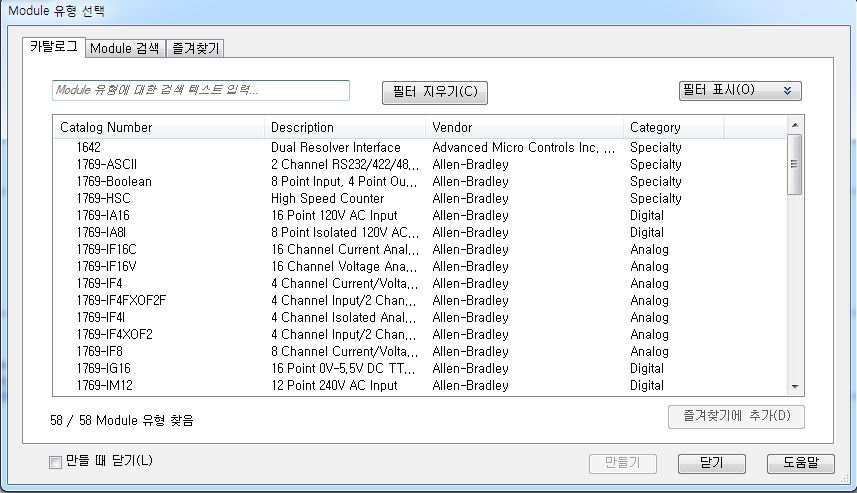
\includegraphics[width=0.9\textwidth]{./picture/module_search.JPG}
 	\caption{
 		Module registration
 	}
 	\label{fig:}
 \end{figure}  
 
 3) 샤시에 설치된 모듈을 검색하여 추가한다.\\
 
 \newpage
 
 위의 과정을 통해서 샷시에 설치된 모듈들을 모두 등록해야만 각 모듈에 해당하는 Tag 정보가 RSLogix5000에 등록되어 해당 모듈을 사용할 수 있다. \
 
 모듈 등록 과정이 끝나면 래더 프로그램을작성하기 위한 설정을 아래와 같이 진행한다.
 
 
 \newpage
 
 \begin{figure}[h]
 	\centering
 	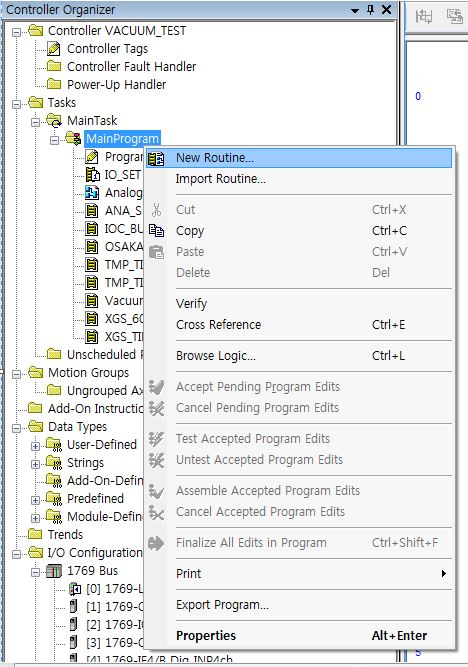
\includegraphics[width=0.7\textwidth]{./picture/new_routine.JPG}
 	\caption{}
 	\label{fig:}
 \end{figure}  
 
  1) Figure 8과 같이 RSLogix5000 좌측 상단부의 Controller Organizer에서 MainProgram $\rightarrow$ NewRoutine 을 선택한다.\\
  
 2) Figure 9처럼 Routine 설정창에 프로그램 이름 및 특성에 대한 내용을 입력한다.\
 Type 메뉴에서 작성할 프로그램 언어를 선택할 수 있다.\\
 
 위의 과정을 통해서 래더 프로그램을 작성하기 위한 준비가 완료되었다.\\

\begin{figure}[h]
	\centering
	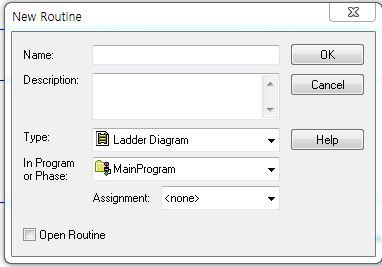
\includegraphics[width=0.7\textwidth]{./picture/routine_setting.JPG}
	\caption{}
	\label{fig:}
\end{figure}  
 

\newpage
 
\section{Ladder Program configuration}\
래더프로그램을 작성하는 방법은 다른 메이커의 PLC와 크게 다르지 않다. 그러나 LS PLC나 미쓰비씨 PLC 등에서 기본적으로 제공되는 Flip Flop 비트 같은 기능은 제공되지 않으므로 같은 기능을 할 수 있는 Routine 프로그램을 구성한 뒤 필요 시 프로그램을 가져와야 한다. 이는 래더 프로그램을 작성하는 사용자의 성향에 따라 불편할 수도 있지만 디폴트 값으로 할당된 메모리가 없으므로 프로그램의 메모리 관리 측면에서는 이득이다.\\

RSLogix5000에서 래더 프로그램을 작성하는 방법을 아래에 간단히 기술한다.    

\begin{figure}[h]
	\centering
	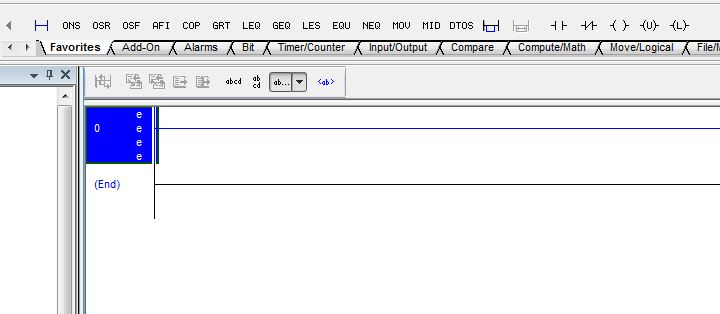
\includegraphics[width=0.95\textwidth]{./picture/menu.JPG}
	\caption{Main screen}
	\label{fig:}
\end{figure}  \

Figure 10은 RSLoigx5000의 메인 화면이다. 화면의 위 쪽은 다른 PLC 프로그램과 마찮가지로 비트 입출력 기호와 명령어들이 나타난다. AB PLC는 자주 쓰는 기호와 명령어들을 Favorites 영역에 추가해서 사용하는 것이 편리하다.

\begin{itemize}
	\item 입출력 구성법
\end{itemize}

\begin{figure}[h]
	\centering
	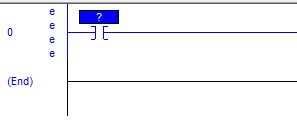
\includegraphics[width=0.6\textwidth]{./picture/input1.JPG}
	\caption{}
	\label{fig:}
\end{figure}  \

1) Figure 10의 상단에서 입력 기호를 클릭해서 Figure 11처럼 해당 래더의 라인에 가져다 놓는다.

\begin{figure}[h]
	\centering
	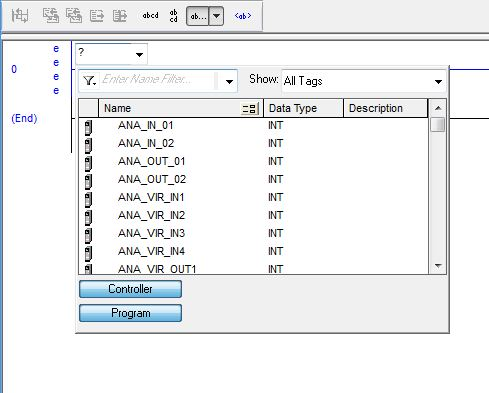
\includegraphics[width=0.6\textwidth]{./picture/input_tag.JPG}
	\caption{}
	\label{fig:}
\end{figure}  \


2) Figure 11의 파란색 물음표 부분을 클릭한 후 Tag 목록에서 사용할 Tag를 선택한다. 

\begin{figure}[h]
	\centering
	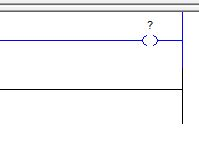
\includegraphics[width=0.4\textwidth]{./picture/coil.JPG}
	\caption{}
	\label{fig:}
\end{figure}  \


3) 위와 같은 방법으로 출력부를 구성한다. 래더 라인에 가져다 놓을 명령어 및 기호들이 데이터 입력의 속성이면 좌측에 구성되고 데이터 출력의 속성이면 우측에 구성이 된다.\\

Figure 14는 출력 속성의 명령어를 래더 라인에 구성한 예이다. 사용된 명령어는 XGS-600에서 측정하고 있는 Vacuum testbed의 Pressure gauge 값으로 기능 및 속성은 시리얼통신 구성방법에서 설명한다.(뒤의 Figure 19와 같음)
 
\begin{figure}[h]
	\centering
	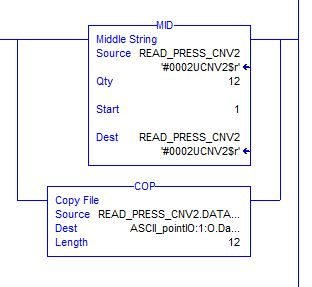
\includegraphics[width=0.6\textwidth]{./picture/ladder_com.JPG}
	\caption{}
	\label{fig:}
\end{figure}  \
 
\newpage

\section{Serial Communication}\
현재 Vacuum testbed 디바이스들 중 PLC와 RS-232 통신을 하는 디바이스는 게이지 컨트롤러인 XGS600과 OSAKA TMP 컨트롤러인 TC-353 이다. 시리얼 통신 구성방법은 명령어만 다를 뿐 동일하므로 XGS-600과의 RS-232 통신 구성을 예를 들어 설명한다.\

 \begin{figure}[h]
 	\centering
 	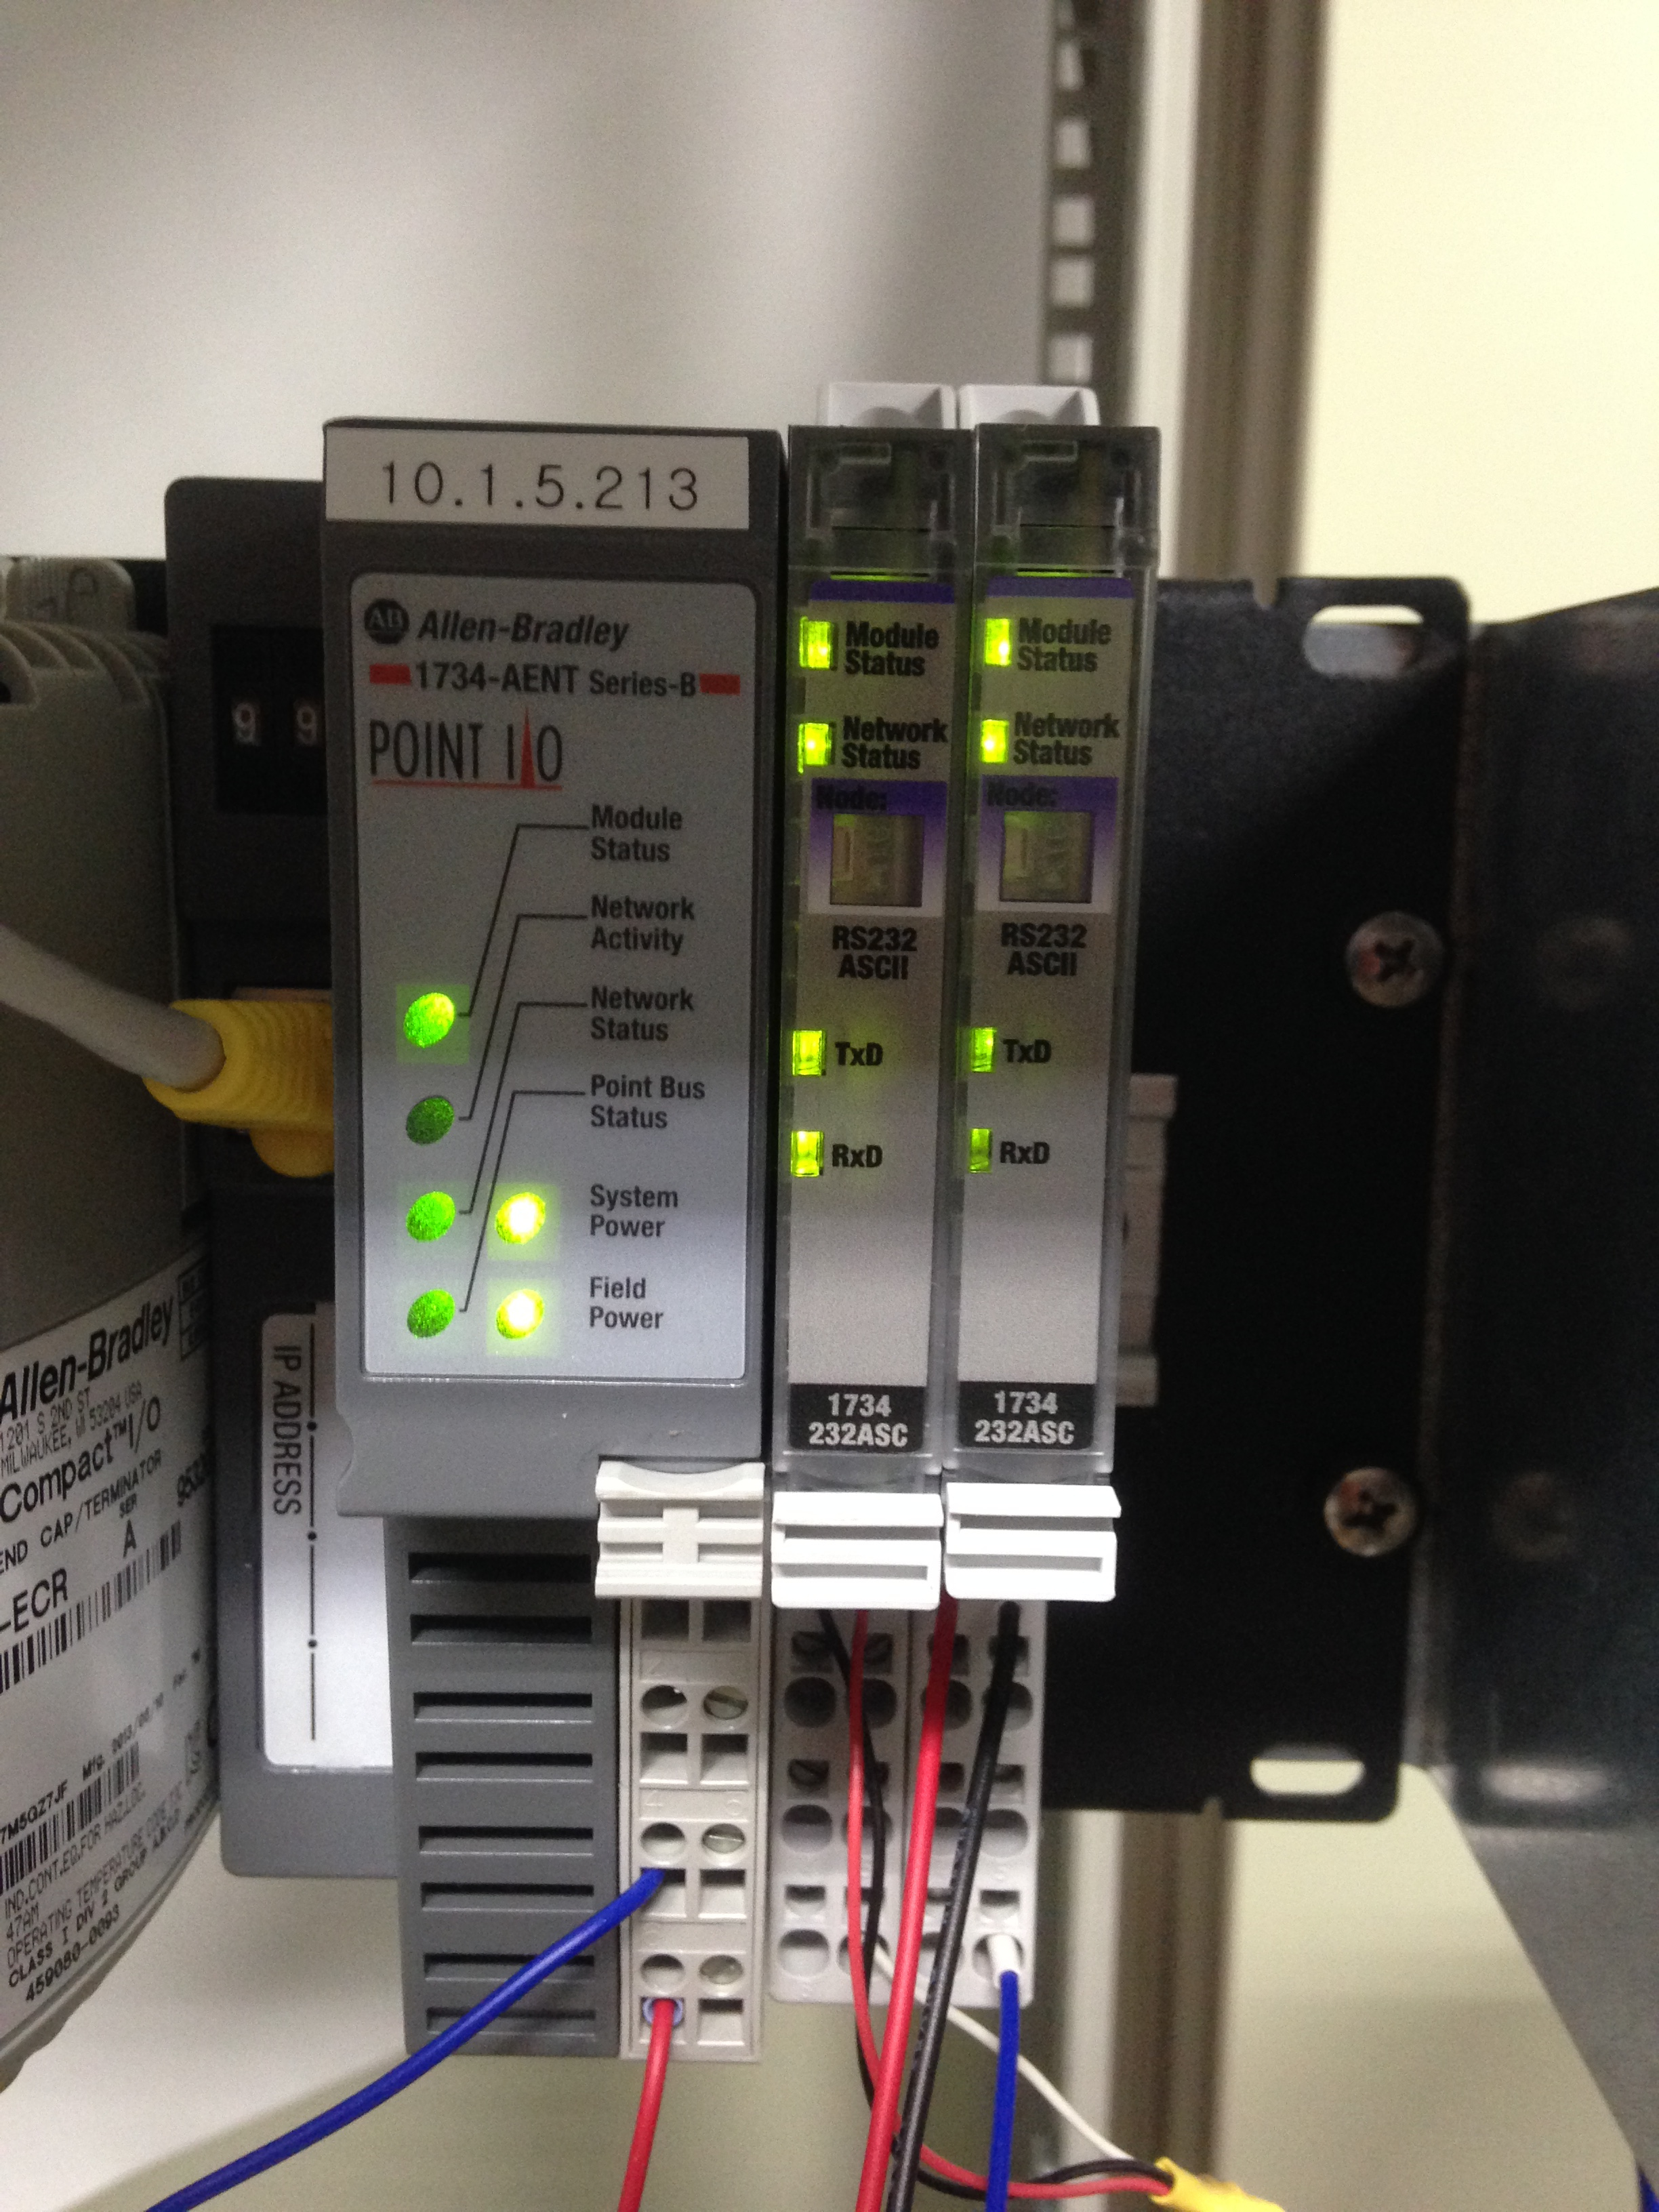
\includegraphics[width=0.6\textwidth]{./picture/pointIO.JPG}
 	\caption{Remote IO module}
 	\label{fig:}
 \end{figure}  \

Figure 15의 모듈은 앞에서 설명한 Point IO 모듈에 시리얼 통신을 위한 1734 232ASC 모델을 2개 장착한 것이다. 각 232ASC 모듚은 XGS-600 및 TC-353의 시리얼 포트와 연결된다.\\

AB PLC에서는 통신을 위한 별도의 소프트웨어 툴은 제공하지 않으며 RSLogix5000에서 모든 설정을 한다. 다른 메이커의 PLC의 경우는 통신을 위한 소프트웨어 툴을 따로 제공해서 클라이언트 측에서 서버 측으로 보내는 데이터를 해당 메모리에 할당한 후 통신 주기를 설정해 주는 방식이다. 데이터 보내기/받기를 위한 별도의 래더 프로그램은 필요 없으며, 그 데이터를 가공하기 위한 래더 프로그램만이 필요한데 반하여 AB PLC의 경우는 데이터 보내기/받기를 위한 설정부터 데이터 가공까지 모두 래더 프로그램으로 구성해야 하는 어려움이 있다. \
주기적으로 명령어를 보내고 응답 메시지를 받는 로직은 프로그램을 구성하는 사용자마다 차이가 있으므로 여기에서는 명령메시지를 가공하는 방법과 받는 메시지를 처리하는 방법을 위주로 설명한다.\\

AB PLC와 XGS-600과의 시리얼 통신의 예를 아래에 기술한다.

\begin{itemize}
	\item 1745-ASC232 데이터 Tag 구성 및 기능
\end{itemize}
		
\begin{figure}[h]
	\centering
	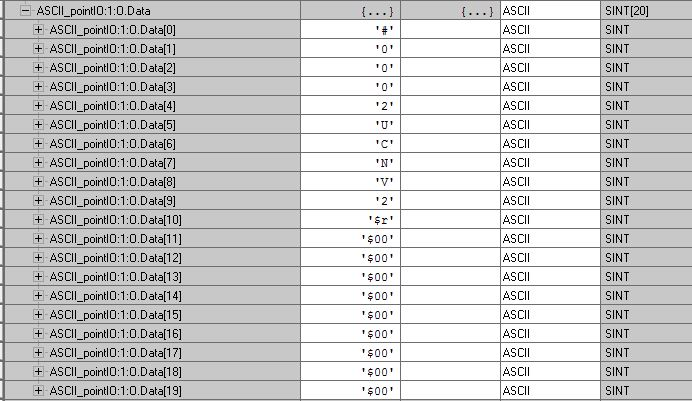
\includegraphics[width=0.95\textwidth]{./picture/sending.JPG}
	\caption{Remote IO Tag}
	\label{fig:}
\end{figure}  

1) Figure 16은 XGS-600 모듈과 연결된 1734 ASC-232 모듈의 출력영역 Tag이다. 그림과 같이 XGS-600측으로 보내는 명령어를 문자로 넣어준다. 위의 예는 XGS-600에 연결된 CNV2라는 이름의 게이지 압력값을 불러오는 명령어이다.\
위의 상태는 PLC측 메모리에 해당 명령어가 입력만 된 상태이다. 이 명령어를 XGS-600측으로 보내기 위해서는 특정 태그 비트를 1스캔 ON 시켜야 한다.\\
	
\begin{figure}[h]
	\centering
	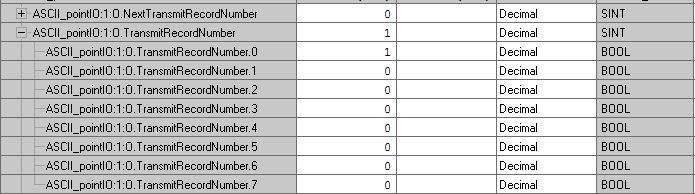
\includegraphics[width=0.95\textwidth]{./picture/transmitbit.JPG}
	\caption{Message sending bit}
	\label{fig:}
\end{figure}

\newpage 

2) Figure 17에서 보이는 데이터 전송비트 Transmit Record Number.0과 Transmit Record Number.1을 1스캔 씩 ON 시키면 '$\sharp$0002UCNV2'라는 명령어가 XGS-600측으로 전달된다.\\

\begin{figure}[h]
 	\centering
 	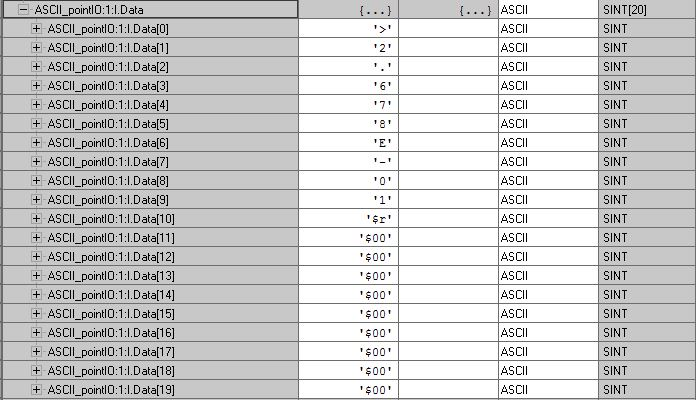
\includegraphics[width=0.95\textwidth]{./picture/receiving.JPG}
 	\caption{Received data}
 	\label{fig:}
\end{figure}
 
3) Figure 18은 XGS-600측에서 보낸 응답메시지를 1734 ASC-232 모듈측 입력영역 Tag로 성공적으로 수신한 상태를 나타내고있다. \\
 
 \newpage
 
1734 ASC-232 모듈로 수신된 메시지는 String 타입으로 PLC 측에서 보내는 명령어에 따라 수신되는 메시지도 다르다. 이 메시지를 UI에서 모니터링 하려면 ASC-232에서 명령어 메시지를 해당 컨트롤러에 보낼 때마다 수신되는 메시지도 다르기 때문에 각각 명령어에 따른 수신메시지를 저장할 Tag도 따로 만들어야 한다. 또한 이 값이 ASC-232에서 보낸 String 형태의 출력값에 따른 String 형태의 입력값이므로 데이터를 비교하기 위해서는 String 형태의 데이터를 Int 형태나 Float 형태의 데이터로 바꾸어 주는 과정이 필요하다. \

앞에서 설명했던 Tag 값에 명령어를 지정하는 방법을 직접 넣지 않고 래더 프로그램을 작성해서 명령어 데이터를 보내고 수신된 메시지를 가공하는 방법을 아래에 기술한다.
 
\begin{itemize}
	\item 래더 프로그램으로 메시지 송수신 하기
\end{itemize} 

\begin{figure}[h]
	\centering
	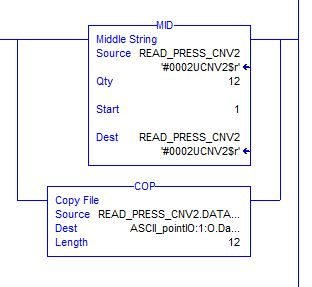
\includegraphics[width=0.5\textwidth]{./picture/ladder_com.JPG}
	\caption{Sending massage}
	\label{fig:}
\end{figure}

1) Figure 19는 String 타입의 명령어 데이터를 만들어서 1734 ASC-232 모듈의 Tag에 할당하는 방법이다.\\

MID 명령어를 이용해서 source 속성에 XGS-600측으로 보낼 명령어를 입력한다.\

Q'ty 속성에는 추출할 문자 갯수를 입력한다.\

Start 속성에는 문자를 추출할 시작 위치를 입력한다.\

Dest 속성에는 추출한 데이터를 보낼 Tag를 입력한다.\\


COP 명령어를 이용해서 Int 타입의 데이터 묶음을 1734 ASC-232 모듈의 Tag로 보낸다.\\

Source 속성에는 String 타입의 첫 번째 Int 타입의 Tag를 입력한다.\

Dest 속성에는 1734 ASC-232의 첫 번째 Int 타입의 Tag를 입력한다.\

Length 속성에는 보낼 Int 타입의 Tag 갯수를 입력한다.\\

위의 예를 설명하면 다음과 같다. 명령어 '$\sharp$0002UCNV2'를 처음부터 12개 잘라서 Int 타입의 데이터로 나눈 뒤 Int 타입의 데이터 12개를 1734 ASC-232 모듈의 Tag로 보내는 과정이다. MID 명령어를 쓴 이유는 래더 프로그램에서 내가 보낼 명령어를 쉽게 바꾸기 위함이다.\\


참고. 본 문서 5장에서 설명한 Digital Output Memory 구조와 마찮가지로 1734 ASC-232 의 String 타입의 Tag는 Sint(Single integer) 형태의 Tag 20개로 나뉜다.

\begin{figure}[h]
	\centering
	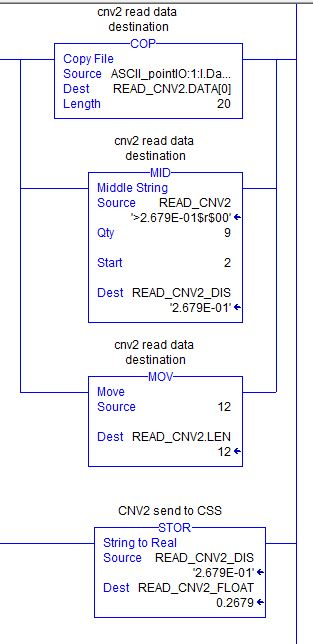
\includegraphics[width=0.5\textwidth]{./picture/read_ladder.JPG}
	\caption{Reading massage}
	\label{fig:}
\end{figure}

\newpage

Figure 20은 XGS-600으로 부터 ASC-232 모듈의 입력 Tag로 수신된 String 형태의 메시지를 모니터링을 위해 해당 Tag로 할당하는 방법이다.\\

COP 명령어를 이용해서 ASC-232 입력 Tag측에 수신된 String 형태의 메시지를 Int형으로 할당된 Tag로 20개 보낸다.\

Source 속성에는 ASC-232의 첫 번째 Int형 Tag를 입력한다.\

Dest 속성에는 데이터 수신을 위해 할당한 String 형태의 Tag 중 첫 번째 Int형 Tag를 입력한다.\

Length 속성에는 보낼 Int 타입의 Tag 갯수를 입력한다.\\

MID 명령어를 이용해서 수신된 데이터를 모니터링을 위해 생성한 Tag로 보낸 후 Float 값으로 가공한다.\

Source 속성에는 수신된 String Tag를 입력한다.\

Q'ty 속성에는 추출할 문자 갯수를 입력한다.\

Start 속성에는 문자 추출을 시작할 위치를 입력한다.\

Dest 속성에는 추출한 문자를 가공할 Tag를 입력한다.\\

STOR 명령어를 이용해서 String 형태의 데이터를 Float의 형태로 가공한다.\

Source 속성에는 변환할 String 형태의 Tag를 입력한다.\

Dest 속성에는 변횐된 데이터가 저장될 Tag를 입력한다.\\

위의 예에서 'READ\_CNV2\_DIS'라는 Tag에 Float 형태로 저장되어 최종적으로 CSS로 꾸며지는 UI에서 모니터링 된다.\\

\begin{figure}[h]
	\centering
	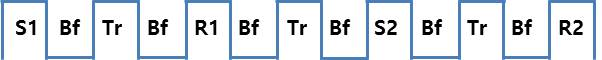
\includegraphics[width=0.5\textwidth]{./picture/timer_bit.jpg}
	\caption{Communication time chart}
	\label{fig:}
\end{figure}

Figure 21은 AB PLC와 XGS-600 및 TC-353과의 데이터 송수신을 위한 Time chart 이다. \
S는 메시지 보내기 신호, Bf는 Buffer, Tr은 Transmit bit, R은 메시지 받기 신호를 말한다.\
각 신호는 Timer로 구성되어 데이터 송수신을 위한 시간 간격을 조절할 수 있다. 

\newpage

\chapter{EPICS IOC 와의 연동}
여기에서는 EPICS IOC와 AB PLC 데이터 교환에 대해서 알아본다. EPICS 환경을 구성하는 방법은 Script\_for\_epics(https://github.com/jeonghanlee/scripts\_for\_epics)를 참조하기 바라며, EPICS IOC와 AB PLC 간의 데이터 통신을 위한 드라이버는 ehter-ip-2-26(ics-web.sns.ornl.gov/kasemir/etherip/)를 사용했다. \\

\section{RELEASE file 설정}
EPICS IOC 생성 후 ~/epics/R3.14.12.5/siteApps/IOC/configure/RELEASE 파일을 다음과 같이 설정한다. 파일의 경로는 PC의 EPICS의 환경에 따라 다르다.\\

\begin{lstlisting}[style=termstyle]

TEMPLATE_TOP=$(EPICS_BASE)/templates/makeBaseApp/top

# If using the sequencer, point SNCSEQ at its top directory:
#SNCSEQ=$(EPICS_BASE)/../modules/soft/seq

# EPICS_BASE usually appears last so other apps can override stuff:
EPICS_BASE=/home/hjson/epics/R3.14.12.5/base

# Set RULES here if you want to take build rules from somewhere
# other than EPICS_BASE:
#RULES=/path/to/epics/support/module/rules/x-y

EHTER_IP=/home/hjson/epics/R3.14.12.5/epicsLibs/synApps_5_8/support/ether_ip-ether_ip-2-26

\end{lstlisting}

RELEASE 파일은 supprot module의 경로를 지정해주는 파일이다. 여기에서는 AB PLC와 EPICS IOC간의 통신을 위한 EtherIP Driver(ether\_ip-ether\_ip-2-26)가 저장되어 있는 경로를 지정해 준다.\

\section{Db Makefile 설정}

Db Makefile은 AB PLC의 Tag를 EPICS IOC의 PV와 일치시키기 위한 db파일을 등록하는 파일이다. Tag의 데이터 형태에 따라 db파일을 생성한 후 Db 디렉토리에 추가해 준다. 현재의 시스템에서의 경로는 '/epics/R3.14.12.5/siteApps/AB\_VACUUM/ABPLCApp/Db/Makefile'이다.\
 
\begin{lstlisting}[style=termstyle]

TOP=../..
include $(TOP)/configure/CONFIG
#----------------------------------------
#  ADD MACRO DEFINITIONS AFTER THIS LINE

#----------------------------------------------------
#  Optimization of db files using dbst (DEFAULT: NO)
#DB_OPT = YES

#----------------------------------------------------
# Create and install (or just install) into <top>/db
# databases, templates, substitutions like this
#DB += xxx.db
DB += abplcDIDO.db
DB += abplcAIAO.db
DB += abplcSTRINGIN.db

\end{lstlisting}

\section{src Makefile 설정}

src Makefile은 support module의 Library 및 dbd 파일의 정보를 등록하는 파일이다. 현재 시스템에서의 경로는 '/epics/R3.14.12.5/siteApps/AB\_VACUUM/ABPLCApb/src/Makefile'이다.\

\begin{lstlisting}[style=termstyle]

TOP=../..

include $(TOP)/configure/CONFIG
#----------------------------------------
#  ADD MACRO DEFINITIONS AFTER THIS LINE
#=============================

#=============================
# Build the IOC application

PROD_IOC = ABPLC
# ABPLC.dbd will be created and installed
DBD += ABPLC.dbd

# ABPLC.dbd will be made up from these files:
ABPLC_DBD += base.dbd

# Include dbd files from all support applications:
#ABPLC_DBD += xxx.dbd

ABPLC_DBD += ether_ip.dbd

# Add all the support libraries needed by this IOC
#ABPLC_LIBS += xxx
ABPLC_LIBS += ether_ip

# ABPLC_registerRecordDeviceDriver.cpp derives from ABPLC.dbd
ABPLC_SRCS += ABPLC_registerRecordDeviceDriver.cpp

# Build the main IOC entry point on workstation OSs.
ABPLC_SRCS_DEFAULT += ABPLCMain.cpp
ABPLC_SRCS_vxWorks += -nil-

# Add support from base/src/vxWorks if needed
#ABPLC_OBJS_vxWorks += $(EPICS_BASE_BIN)/vxComLibrary

# Finally link to the EPICS Base libraries
ABPLC_LIBS += $(EPICS_BASE_IOC_LIBS)

#===========================

include $(TOP)/configure/RULES
#----------------------------------------
#  ADD RULES AFTER THIS LINE



\end{lstlisting}


\section{Record file 작성}

Record file은 AB PLC에서 사용되고 있는 Tag를 EPICS IOC PV와 일치시키기 위해 작성하는 파일이다. EPICS record file을 작성하는 Reference를 EPICS 홈페이지에서 확인할 수 있다. 다음은 현재 시스템에서 사용한 OSAKA TMP 컨트롤러 및 XGS-600 컨트롤러의 제어를 위해 생성한 AB PLC의 Tag를 데이터 형태에 따라 나누어 작성한 파일들의 일부이다.\\

아래의 record file은 Digital Input/Output 값을 제어하기 위한 파일이다. 현재 시스템에서의 경로는 '/epics/R3.14.12.5/siteApps/AB\_VACUUM/ABPLCApp/Db/abplcDIDO.db'이다.\\

\begin{lstlisting}[style=termstyle]

record(bi, "$(IOC):TMP_ACCEL")
{
field(SCAN, ".1 second")
field(INP, "@$(PLC) TMP_ACCEL")
field(DTYP, "EtherIP")
field(ZNAM, "False")
field(ONAM, "True")
}

record(bi, "$(IOC):TMP_NORMAL")
{
field(SCAN, ".1 second")
field(INP, "@$(PLC) TMP_NORMAL")
field(DTYP, "EtherIP")
field(ZNAM, "False")
field(ONAM, "True")
}

record(bi, "$(IOC):TMP_ERROR")
{
field(SCAN, ".1 second")
field(INP, "@$(PLC) TMP_ERROR")
field(DTYP, "EtherIP")
field(ZNAM, "False")
field(ONAM, "True")
}

record(bi, "$(IOC):TMP_BRAKE")
{
field(SCAN, ".1 second")
field(INP, "@$(PLC) TMP_BRAKE")
field(DTYP, "EtherIP")
field(ZNAM, "False")
field(ONAM, "True")
}

record(bi, "$(IOC):TMP_RMT_STATUS")
{
field(SCAN, ".1 second")
field(INP, "@$(PLC) TMP_RMT_STATUS")
field(DTYP, "EtherIP")
field(ZNAM, "False")
field(ONAM, "True")
}

\end{lstlisting}

	 	
아래의 record file은 Analog Input/Output 값을 제어하기 위한 파일이다. 현재 시스템에서의 경로는 '/epics/R3.14.12.5/siteApps/AB\_VACUUM/ABPLCApp/Db/abplcAIAO.db'이다.\\


\begin{lstlisting}[style=termstyle]

record(ai, "$(IOC):CNV2_READ")
{
field(DESC, "CNV_GAUGE VALUE")
field(SCAN, ".1 second")
field(INP, "@$(PLC) READ_CNV2_FLOAT")
field(DTYP, "EtherIP")
}

record(ai, "$(IOC):AUX2_READ")
{
field(DESC, "AUX_GAUGE VALUE")
field(SCAN, ".1 second")
field(INP, "@$(PLC) READ_AUX2_FLOAT")
field(DTYP, "EtherIP")
}


## Belows are setting for OSAKA TMP controller analog signal

record(ai, "$(IOC):TOTAL_TIME1")
{
field(DESC, "TMP_OPERATING TIME")
field(SCAN, ".1 second")
field(INP, "@$(PLC) READ_TIME_DINT")
field(DTYP, "EtherIP")
}


## Belows are settign to read the analog moudle value of AB PLC.

record(ai, "$(IOC):AI_CH0")
{
field(DESC, "Channel 0 Input value")
field(SCAN, ".1 second")
field(INP, "@$(PLC) Local:4:I.Ch0Data")
field(DTYP, "EtherIP")

}

record(ai, "$(IOC):AI_CH1")
{
field(DESC, "Channel 1 Input value")
field(SCAN, ".1 second")
field(INP, "@$(PLC) Local:4:I.Ch1Data")
field(DTYP, "EtherIP")
}

\end{lstlisting}

아래의 record file은 String 값을 제어하기 위한 파일이다. 현재 시스템에서의 경로는 '~/epics/R3.14.12.5/siteApps/AB\_VACUUM/ABPLCApp/Db/STRINGIN.db'이다.\\
		
\begin{lstlisting}[style=termstyle]

record(stringin, "$(IOC):CNV2_value")
{
field(DESC, "CNV2_PRESSURE")
field(SCAN, ".5 second")
field(INP, "@$(PLC) READ_CNV2_DIS")
field(DTYP, "EtherIP")
}

record(stringin, "$(IOC):AUX2_value")
{
field(DESC, "AUX2_PRESSURE")
field(SCAN, ".5 second")
field(INP, "@$(PLC) READ_AUX2_DIS")
field(DTYP, "EtherIP")
}

\end{lstlisting}

\section{st.cmd file 작성}

st.cmd 파일은 EPICS IOC를 실행하는 파일이다. AB PLC의 주소 및 데이터를 송수신하는 buffer 크기 등을 설정해 준다.\\

\begin{lstlisting}[style=termstyle]

#!../../bin/linux-x86_64/ABPLC

## You may have to change ioc to something else
## everywhere it appears in this file

< envPaths

cd "${TOP}"

## Register all support components
dbLoadDatabase "dbd/ABPLC.dbd"
ABPLC_registerRecordDeviceDriver pdbbase

## Load record instances
## dbLoadTemplate "db/userHost.substitutions"
## dbLoadRecords "db/dbSubExample.db", "user=hjsonHost"

dbLoadRecords("db/abplcDIDO.db","PLC=AB, IOC=ABPLC")
dbLoadRecords("db/abplcAIAO.db","PLC=AB, IOC=ABPLC")
dbLoadRecords("db/abplcSTRINGIN.db","PLC=AB, IOC=ABPLC")

## Set this to see messages from mySub
#var mySubDebug 1

## Run this to trace the stages of iocInit
#traceIocInit

EIP_buffer_limit(500)

drvEtherIP_init()

drvEtherIP_define_PLC("AB","10.1.5.204",0)

cd "${TOP}/iocBoot/${IOC}"
iocInit


\end{lstlisting}

\newpage

\chapter{User Interface 구성}
	
현재 Demo Vacuum System의 UI는 Control System Studio(CSS)로 구성되어 있다. UI에서 EPICS IOC를 통해 시스템을 제어하는 변수는 아래와 같다.\\

\begin{itemize}
	
	\item Gate valve ON/OFF and status monitoring 
	\item ANGLE valve ON/OFF and status monitoring	 
	\item Convection gauge monitoring (XGS-600)
	\item Full range gauge monitoring (XGS-600)
	\item Reading unit setting (XGS-600)
	\item TMP remote start/stop (TC-353)
	\item TMP status monitoring (TC-353)
	
\end{itemize}

\begin{figure}[h]
	\centering
	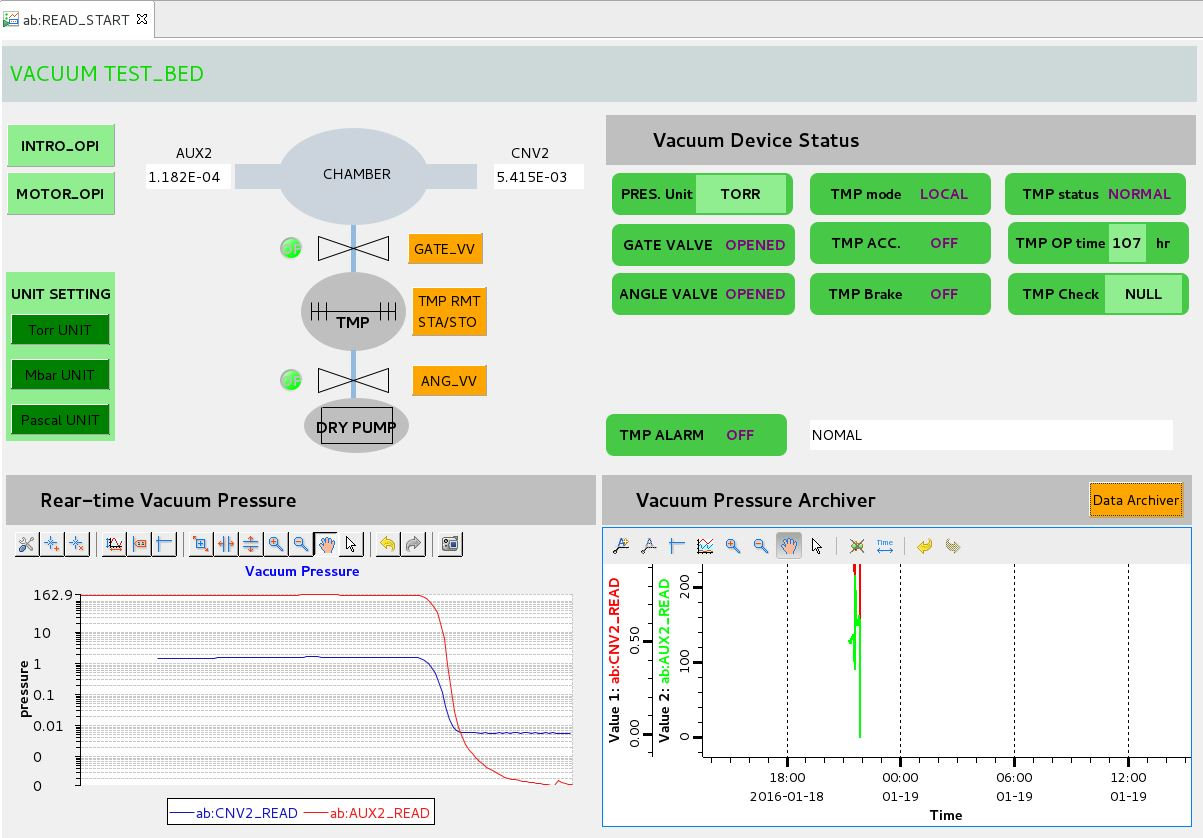
\includegraphics[width=1\textwidth]{./picture/UI1.JPG}
	\caption{UI configuration}
	\label{fig:}
\end{figure}

현재 Demo Vacuum Ststem의 Chamber 진공도는 2채널로 구성되어 0.5초 간격으로 각 채널의 정보를 모니터링 하고 있으며, TMP의 상태정보 또한 일정한 시간 간격으로 각 채널에 대한 정보를 모니터링 하고 있다. Quick appliance를 실행하여 일주일 단위로 진공도 및 EPICS IOC PV 데이터를 저장할 수 있게 구성하였다. 현재 시스템은 Rough Line, Fore Line에 대한 구분이 없고, 단순한 구성이므로 별도의 인터락 및 순차제어에 대한 로직은 구성하지 않았다. 추후 중이온가속기의 진공 시스템이 AB PLC로 구성될 시에는 사용되는 게이지 및 펌프에 따라 통신환경을 구성할 수 있도록 본 문서를 지속적으로 업데이트 할 예정이다.   

\end{document}
